\documentclass{article}
\usepackage[margin=0.8in]{geometry}
\usepackage{graphicx}
\usepackage{amsmath, amssymb, hyperref, bm}

\renewcommand{\thesection}{\arabic{section}.}
\renewcommand{\thesubsection}{\thesection\arabic{subsection}.}

\setlength{\parindent}{0pt}
\setlength{\parskip}{0.5em}

\title{Control System Analysis\\of the \textit{Triangle}}
\author{\texttt{dc\&e}}
\date{May 1, 2025\footnote{Last compiled: \today\hfill\texttt{id: 24003}}}
\begin{document}

\maketitle

\tableofcontents


\newpage

\section*{Preface}

This work was carried out by \texttt{dc\&e}, with contributions from:

\begin{enumerate}
  \item Himanshu Paudel
\end{enumerate}

\newpage

\section{Introduction}

We present the mathematical modeling, control system design, and theoretical analysis of the \textit{Triangle} balance robot.

\section{Differential equations the \textit{Triangle}}

In this section, we develop the mathematical model of the \textit{Triangle}, i.e., derive its differential equations. These equations form the basis for stability analysis, control design, and simulation of the control system.

\begin{figure}[ht]
  \centering
  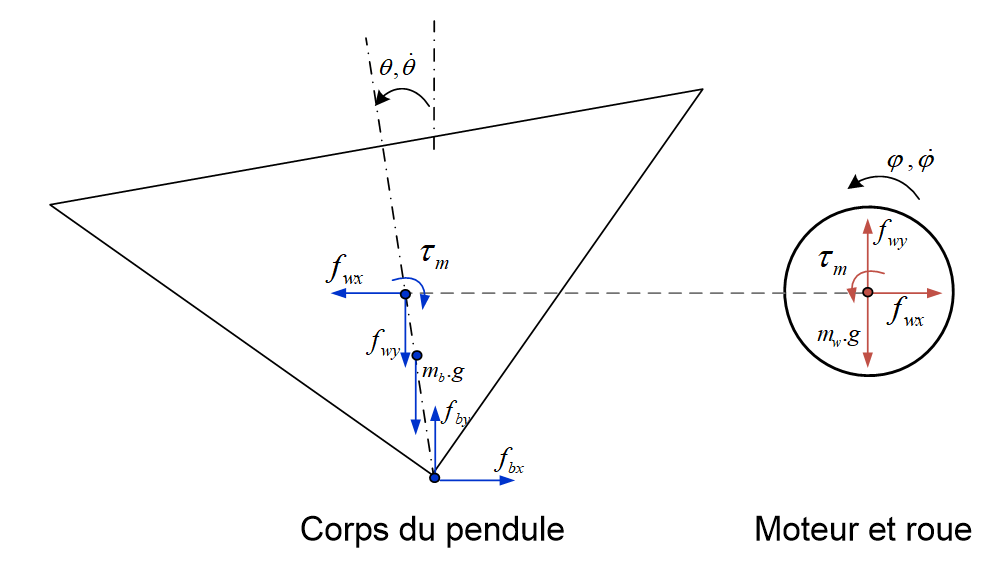
\includegraphics[scale=0.24]{triangle.png}
  \caption{Forces and torques acting on the \textit{Triangle} Balance. Figure stolen from \cite{ipendulum}}
  \label{fig_triangle}
\end{figure}

Fig.(\ref{fig_triangle}) shows the free-body diagram of the \textit{Triangle} where the parameters are defined as following:

\begin{align*}
  \theta &= \text{Pendulum angle} \\
  \varphi &= \text{Wheel angle relative to pendulum} \\
  m_b, I_b, l_b &= \text{Mass, inertia, and center of mass height of pendulum body} \\
  m_w, I_w, l_w &= \text{Mass, inertia, and center of mass height of wheel} \\
  \tau_m &= \text{Motor torque} \\
  \tau_f &= \text{Friction torque} \\
  M &= m_b l_b + m_w l_w \\
  I &= I_b + m_b l_b^2 + m_w l_w^2
\end{align*}

\subsection{Construction of the Lagrangian}

Euler-Lagrange equation is used to derive the differential equation, threfore, we start by expressing the Kinetic energy $T$ and potential energy $V$ of the \textit{Triangle} to compute the Lagrangian as
\begin{equation}
  \label{eqn_lagrangian}
  L=T-V
\end{equation}

The kinetic energy of the \textit{Triangle} is the sum of kinetic energy of the body $T_{b}$, and that of the wheel $T_{w}$. The term $T_{b}$ can be expressed at the sum of the kinetic energy due to the angular motion and the translational motion of the body's center of mass i.e.
\begin{equation}
  T_b=\dfrac{1}{2}\left(I_{b} + m_{b} l_{b}^{2}\right)\dot{\theta}^{2}
\end{equation}

where, $l_{b}\dot{\theta}$ is the linear velocity of the center of mass.\footnote{If a rigid body rotates around a fixed point with angular velocity $\dot{\theta}$, any point on the body located at a distance $r$ from the pivot traces a circular path. The linear velocity $v$ of that point is related to the angular velocity as $v=r\dot{\theta}$.}

The, reaction wheel, on the other hand, has three sources of its kinetic energy: (1) rotation about its own axis, (2) rotation of the body about its axis, and (3) translational motion in space with respect to the inertial frame as the body rotates. Therefore, the kinetic energy of the wheel is the sum of its rotational and the translational kinetic energies i.e.

\begin{equation}
  T_w=\dfrac{1}{2}\left(I_{w}(\dot{\theta}+\dot{\varphi})^{2}+m_{w}l_{w}^{2}\dot{\theta}^2\right).
\end{equation}

The total kinetic energy of the \textit{Triangle} can be expressed as
\begin{equation}
  \begin{split}
    T&=T_{b}+T_{w}\\
    &=\dfrac{1}{2}\left(I_{b} + m_{b} l_{b}^{2}\right)\dot{\theta}^{2}+\dfrac{1}{2}\left(I_{w}(\dot{\theta}+\dot{\varphi})^{2}+m_{w}l_{w}^{2}\dot{\theta}^2\right)\\
    &= \frac{1}{2}\left(\left(I_b+m_{b}l_{b}^{2}+I_{w}+m_{w}l_{w}^{2}\right)\dot{\theta}^2+2I_{w}\dot{\theta}\dot{\varphi}+I_{w}\dot{\varphi}^2\right)\\
    &= \frac{1}{2}\left(I\dot{\theta}^2+I_{w}\dot{\theta}^{2}+2I_{w}\dot{\theta}\dot{\varphi}+I_{w}\dot{\varphi}^2\right)\\
    &= \frac{1}{2}\left(I\dot{\theta}^{2}+I_{w}(\dot{\theta}+\dot{\varphi})^{2}\right)
  \end{split}
\end{equation}

where, $I=I_b+m_{b}l_{b}^{2}+m_{w}l_{w}^{2}$.

We know that a mass' potential energy depends on its vertical position (the good old $-mgh$). Both the body and the wheel rotates with the same angle $\theta$ with respect to the vertical. Therefore, as the body rotates, both center of mass move in a circular arc of radius $l_{b}$ and $l_{w}$ respectively. The vertical height of each center of mass relative to the pivot is:
\begin{equation*}
  \begin{split}
    h_{b}&=-l_{b}\cos\theta\\
    h_{w}&=-l_{w}\cos\theta
  \end{split}
\end{equation*}

where the terms are negative because $\theta=0$. The total potential energy is the \textit{Triangle} the sum of potential enrgies of the body and the wheel, i.e.
\begin{equation}
  \begin{split}
    V&=-m_{b}gh_{b}-m_{w}gh_{w}\\
    &=-(m_{b}gl_{b}+m_{w}gl_{w})\cos\theta\\
    &=-Mg\cos\theta
  \end{split}
\end{equation}

where, $M=m_{b}l_{b}+m_{w}l_{w}$.

We can now use Eqn.(\ref{eqn_lagrangian}) to compute the Lagrangian.

\begin{equation}
  L=T-V=\frac{1}{2}I\dot{\theta}^{2}+\dfrac{1}{2}I_{w}(\dot{\theta}+\dot{\varphi})^{2}+Mg\cos\theta
\end{equation}

\subsection{Equations of motion}

\subsubsection*{Equation of motion of the body}

The Euler-Lagrange equation for the body is expressed as
\begin{equation}
  \label{eqn_elb}
  \dfrac{d}{dt}\left( \dfrac{\partial L}{\partial\dot{\theta}} \right)-\dfrac{\partial L}{\partial\theta}=\tau_{f}-\tau_{m}.
\end{equation}

Computing the terms involved.
\begin{equation}
  \begin{split}
    \dfrac{\partial L}{\partial\dot{\theta}}&=I\dot{\theta}+I_{w}(\dot{\theta}+\dot{\varphi})
    \implies\dfrac{d}{dt}\left(\dfrac{\partial L}{\partial\dot{\theta}}\right)=(I+I_{w})\ddot{\theta}+I_{w}\ddot{\varphi}\\
    \dfrac{\partial L}{\partial\theta}&=-Mg\sin\theta
    \end{split}
\end{equation}

Plugging in the terms to Eqn.(\ref{eqn_elb}), we get the equation of motion of the body.

\begin{equation}
  \label{eqn_tempb}
  (I+I_{w})\ddot{\theta}+I_{w}\ddot{\varphi}+Mg\sin\theta=\tau_{f}-\tau_{m}
\end{equation}

\subsubsection*{Equation of motion of the wheel}

The Euler-Lagrange equation for the wheel is expressed as
\begin{equation}
  \label{eqn_elw}
  \dfrac{d}{dt}\left(\dfrac{\partial L}{\partial\dot{\varphi}} \right)-\dfrac{\partial L}{\partial\varphi}=\tau_{f}-\tau_{m}.
\end{equation}

Similar to what we did for the body, computing the terms involved,

\begin{equation}
  \begin{split}
  \dfrac{\partial L}{\partial \dot{\varphi}}&=I_w (\dot{\theta} + \dot{\varphi})\implies\dfrac{d}{dt}\left(\dfrac{\partial L}{\partial\dot{\varphi}} \right)=I_{w}(\ddot{\theta}+\ddot{\varphi})\\
  \dfrac{\partial L}{\partial\varphi}&=0
  \end{split}
\end{equation}

Plugging the expression into the Eqn.(\ref{eqn_elw}), we get

\begin{equation}
  \label{eqn_tempw}
  \begin{split}
    I_{w}(\ddot{\theta}+\ddot{\varphi})&=\tau_{m}-\tau_{f}\\
    \implies\ddot{\varphi}&= \dfrac{\tau_m - \tau_f}{I_w} - \ddot{\theta}\\
  \end{split}
\end{equation}

\subsubsection*{Equations of motion of the system}

We can observe that equation of motion of both body and the wheel are coupled with double derivatives as both Eqn.(\ref{eqn_tempb}) and  Eqn.(\ref{eqn_tempw}) contains both terms $\ddot{\theta}$ and $\ddot{\varphi}$. Now we will derive separate equation of motion for each of them by decoupling the double derivative terms.

We begin by plugging Eqn.(\ref{eqn_tempw}) into Eqn.(\ref{eqn_tempb}).

\begin{equation}
  \begin{split}
    \label{eqn_eomb}
    (I+I_{w})\ddot{\theta}+I_{w}\left(\dfrac{\tau_{m}-\tau_{f}}{I_{w}}-\ddot{\theta}\right)+Mg\sin\theta&=\tau_{f}-\tau_{m}\\
  I\ddot{\theta}=Mg\sin\theta-\tau_{m}+\tau_{f}\\
  \implies\ddot{\theta}=\dfrac{Mg\sin\theta-\tau_{m}+\tau_{f}}{I}
  \end{split}
\end{equation}

Plugging the expression in Eqn.(\ref{eqn_tempw}) gives us

\begin{equation}
  \label{eqn_eomw}
  \ddot{\varphi} = \dfrac{(I + I_w)(\tau_m - \tau_f)}{I I_w} - \dfrac{M g \sin\theta}{I}
\end{equation}

Eqn.(\ref{eqn_eomb}) and Eqn.(\ref{eqn_eomb}) are the equations of motion of the \textit{Triangle}.

\subsection{First order form}
\begin{center}
  TODO
\end{center}

\newpage
\section{Stability analysis and controller design}

The goal of this section is to design control law for the \textit{Triangle} by using the mathematical tools of the control theory by trying our best to prove our assumptions so that we are comfortable with what we believe.

The goal of the controller is to regulate $\theta$,  $\dot{\theta}$, and $\dot{\varphi}$ to zero. We're not concerned with $\varphi$ at the moment—that's something for a future project. We will begin by performing mathematical analysis proving why we cannot have smooth single control law which can swing up and balance the \textit{Triangle}. That being done, we are naturally lead to implementing two controllers, one for the swing-up and the next for stabilization. Each of them are discussed in detail. Finally, the question of when to switch from swing-up to stabilization is addressed.

\subsection{A global asymptotic controller}

In this section we apply Brockett's condition to check if a single global asymptotic controller can do the job of balancing the \textit{Triangle} from any initial condition.
\begin{center}
  TODO
\end{center}

\subsection{Stabilizer}

\subsubsection*{Lyapunov function}

Since we are interested only on $\theta$,  $\dot{\theta}$, and $\dot{\varphi}$, we design an energy like Lyapunov function

\begin{equation}
  V = \frac{1}{2} I \dot{\theta}^2 + MgL (1 - \cos\theta) + \frac{1}{2} k_1 \dot{\varphi}^2, \quad k_1 > 0
\end{equation}

where the first two terms represents the mechanical energy of robot body. We synthesize the third, wheel damping, term as we are interested in the angular rate of the wheel as well. The term $k_{1}$ represents the magnitude of damping. It should be noted that we do not require custom gains on other terms ($I$, $M$, $g$, and $L$) because they are provided by physics and system parameters.

Following the steps of Lyapunov analysis, now we compute the time derivative $V$, and plug in the expressions from the equations of motion Eqn.(\ref{eqn_eomb}) and Eqn.(\ref{eqn_eomw}).

\begin{align}
  \dot{V} &= I \dot{\theta} \ddot{\theta} + MgL \dot{\theta} \sin\theta + k_1 \dot{\varphi} \ddot{\varphi} \nonumber \\
          &= \dot{\theta}(2MgL \sin\theta - \tau_m) + k_1 \dot{\varphi}\left(\frac{(I + I_w)}{I I_w}\tau_m - \frac{MgL \sin\theta}{I}\right)
  \label{eqn_vdot}
\end{align}

We now, \textit{search for} the control law forces $\dot{V}$ to be negative semi-definite i.e. $\dot{V}\leq0$.

\begin{equation}
  \tau_m = 2MgL \sin\theta + k_2 \dot{\theta} - \tau_{f}- k_1 \frac{(I + I_w)}{I I_w} \dot{\varphi}
  \label{eqn_ctrl}
\end{equation}

Plugging in the expression of control torque into Eqn.{\ref{eqn_vdot}} to make sure if is $\dot{V}$ indeed negative semi-definite.

\begin{equation}
  \dot{V} = -k_2 \dot{\theta}^2 - k_1 \frac{(I + I_w)^2}{I^2 I_w^2} \dot{\varphi}^2 \leq 0
\end{equation}

When $\dot{V}$ is negative semi-definite, we ask LaSalle for help!

\subsubsection*{LaSalle's invariance principle}

LaSalle's principle requires finding the largest invariant set where $\dot{V} = 0$:

\begin{enumerate}
  \item From \eqref{eqn_vdot}, $\dot{V} = 0$ implies $\dot{\theta} = 0$ and $\dot{\phi} = 0$

  \item Substituting $\dot{\theta} = \dot{\phi} = 0$ into \eqref{eqn_eomb} and \eqref{eqn_eomw}:
  \begin{align}
    0 &= MgL\sin\theta - \tau_m \label{eq:theta_eq} \\
    0 &= \frac{(I + I_w)\tau_m}{I I_w} - \frac{MgL\sin\theta}{I} \label{eq:phi_eq}
  \end{align}

  \item Substituting the control law \eqref{eqn_ctrl} with $\dot{\theta} = \dot{\phi} = 0$:
  \begin{equation}
    \tau_m = 2MgL\sin\theta
  \end{equation}

  \item Combining with \eqref{eq:theta_eq}:
  \begin{equation}
      MgL\sin\theta = 2MgL\sin\theta \implies \sin\theta = 0
  \end{equation}
\end{enumerate}

The only invariant solutions are:
\begin{enumerate}
   \item$\theta=0,\dot{\theta}=0,\dot{\phi}=0$ (desired upright equilibrium)
   \item$\theta=\pi,\dot{\theta}=0,\dot{\phi}=0$ (unstable downward position)
\end{enumerate}

Since $V$ is radially unbounded and the downward position is unstable, all trajectories converge to the upright equilibrium $(\theta, \dot{\theta}, \dot{\phi}) = (0, 0, 0)$.

\subsubsection*{The stabilizer control law}

Our controller, in nonlinear form, as expressed in Eqn.(\ref{eqn_ctrl}) is
\begin{equation*}
  \tau_m=2MgL\sin\theta+k_{2}\dot{\theta}-\tau_{f}-k_1\frac{(I+I_w)}{II_w}\dot{\varphi}
\end{equation*}

The first term compensates gravity, second damps the robot velocity, third compensates friction, and the last damps the wheel velocity. If we are near the equilibrium angle, then gravity compensation can be considered linear with the approximation $\sin\theta\approx\theta$ which linearizes the control law to be
\begin{equation}
  \tau_m=k_{p}\theta+k_d\dot{\theta}+k_{w}\dot{\varphi}-\tau_{f}.
\end{equation}

This requires us to determine the friction of the motor. However, the classic action of neglecting friction leads to simpler linear control law
\begin{equation}
  \tau_m=k_{p}\theta+k_d\dot{\theta}+k_{w}\dot{\varphi}
\end{equation}

where, $k_{p}=2MgL$, $k_{d}=k_{2}$, and $k_{w}=-k_{1}(I+I_w)/(II_{w})$.

\subsection{Swing-up controller}

\begin{center}
  TODO
\end{center}

\subsection{Region of convergence}

In this section, we address the critical question:
\begin{quote}
  ``\textit{When should the controller switch from swing-up to stabilization?}''
\end{quote}

\begin{center}
  TODO
\end{center}

\bibliographystyle{plain}
\bibliography{references}

\end{document}
